\chapter{Architektura proponowanego systemu}
\label{cha:architektura}

{\it

W ramach projektu przeprowadzono analizę wykorzystania mechanizmów wprowadzonych przez koncepcję systemów zarządzania tożsamościami dla różnych typów zastosowań. W tym celu zaproponowana została architektura dla przykładowych aplikacji. Jako specyfikację realizującą założenia systemów zarządzania tożsamościami wybrano standard SAML. Punktem wyjścia dla projektu było wdrożenie koncepcji jednokrotnego uwierzytelniania dla aplikacji webowych. Głównym elementem architektury systemu umożliwiającym tą funkcjonalność jest usługa ,,Identity Provider'' - potwierdzająca tożsamość użytkownika. Następnym krokiem było rozszerzenie mechanizmów uwierzytelniania opartych o protokół SAML na serwisy webowe. Zaproponowano architekturę systemu umożliwiającą uwierzytelnianie klientów usług webowych niezależnie od standardu dostarczania usług(np. SOAP lub REST) przy użyciu protokołu SAML. Głównym elementem architektury dla tego typu systemów jest usługa ,,Security Token Service'' - przydzielająca klientom tokeny potwierdzające ich tożsamość. 

Zastosowanie mechanizmów bezpieczeństwa protokołu SAML w architekturze zorientowanej na usługi zostało przeanalizowane na przykładzie prototypu systemu dokonywania zamówień w sklepie internetowym. Opracowano architekturę systemu składającego się z usług obsługujących różne etapy dokonywania zamówienia - sprawdzanie dostępności produktu, zlecenie przygotowania towaru do wydania, zlecenie dostawy, rejestracja transakcji w serwisie księgowym. Usługi  mogą być dostarczane przy zastosowaniu różnych standardów. Architektura systemu uwzględnia również wprowadzenie dodatkowej warstwy pośredniczącej w dostępie do serwisów - magistrali usług. Opracowano także model procesu biznesowego opisujący przebieg dokonywania zamówienia przy użyciu dostępnych usług. 

}

%---------------------------------------------------------------------------

\autsection{Podział na komponenty}{Krzysztof Wilaszek}
\label{sec:komponenty}

	\subsection{Komponenty architektury aplikacji webowych z mechanizmem jednokrotnego uwierzytelniania}

		\begin{figure}[h]
			\centering
			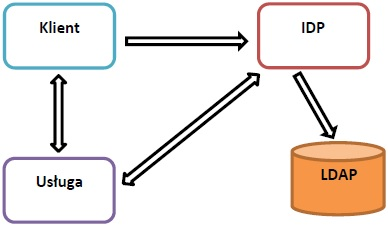
\includegraphics{img/samlWeb.jpg}
			\caption{Jednokrotne uwierzytelnianie aplikacji webowych w protokole SAML}
			\label{webSSO}
		\end{figure}

		Podstawowym elementem pozwalającym na realizację procedury jednokrotnego uwierzytelniania dla aplikacji webowych jest usługa ,,Identity Provider''. Usługa odpowiada za uwierzytelnianie klientów oraz dostarcza tożsamości użytkowników do zaufanych aplikacji. IdP wykorzystuje usługę katalogową LDAP jako bazę tożsamości. Dostawcy usług weryfikują tożsamość klienta żądającego dostępu do zasobów. Gdy konieczne jest uwierzytelniania - polegają na mechanizmach dostarczanych przez usługę IdP. Klient komunikuje się z usługą IdP w procesie uwierzytelniania przesyłając dane potwierdzające jego tożsamość.

	\subsection{Komponenty systemu uwierzytelniania klientów usług webowych w oparciu o standard SAML}

		\begin{figure}[h]
			\centering
			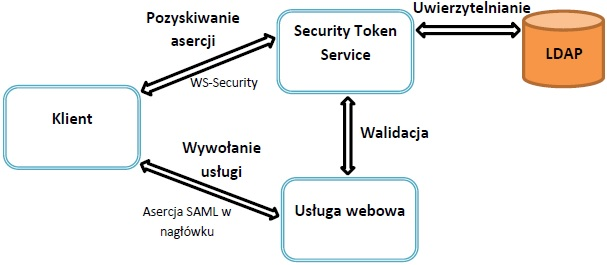
\includegraphics{img/samlWS.jpg}
			\caption{Uwierzytelnianie klienta serwisu webowego z wykorzystaniem SAML}
			\label{Uwierzytelnianie klienta serwisu webowego z wykorzystaniem SAML}
		\end{figure}

		Implementacja mechanizmu uwierzytelniania dla klientów usług webowych powinna korzystać z rozwiązań wprowadzonych przez standard WS-Trust. W skład infrastruktury systemu wchodzi usługa ,,Security Token Service'' odpowiedzialna za uwierzytelnianie użytkowników i generowanie asercji SAML. Serwis korzysta z bazy użytkowników udostępnianej np. przez usługę katalogową LDAP. Dzięki serwisowi STS klient pozyskuje token bezpieczeństwa - asercję SAML, która może być przekazywana do usługi, do której użytkownik chce uzyskać dostęp. Klient dokonuje procesu uwierzytelniania jednokrotnie - raz pozyskana asercja może zostać wykorzystana wielokrotnie dla różnych usług w celu potwierdzenia tożsamości klienta. Mechanizm uwierzytelniania klienta i pozyskiwania asercji korzysta ze specyfikacji WS-Security - użytkownik przekazuje do usługi STS swoje dane uwierzytelniające(identyfikator i hasło); gdy dane są poprawne usługa zwraca token bezpieczeństwa. Otrzymana asercja przekazywana jest w nagłówku SOAP lub HTTP(dla usług typu REST) do wywoływanych serwisów.

		Udostępniając usługi webowe, których zasoby powinny być chronione należy zagwarantować skuteczność kontroli dostępu do serwisu. Żaden nieuwierzytelniony lub nieuprawniony użytkownik nie powinien uzyskać praw dostępu do któregokolwiek z zasobów. Jednym z rozwiązań tego problemu jest centralizacja punktu uwierzytelniania i autoryzacji klientów serwisów - obsługa każdego otrzymanego żądanie użytkownika powinna rozpoczynać się od weryfikacji uprawnień klienta do pozyskiwanych zasobów. Rozwiązanie tego typu opisywane jest przez wzorzec ,,Message Interceptor Gateway''. 

		\begin{figure}[h]
			\centering
			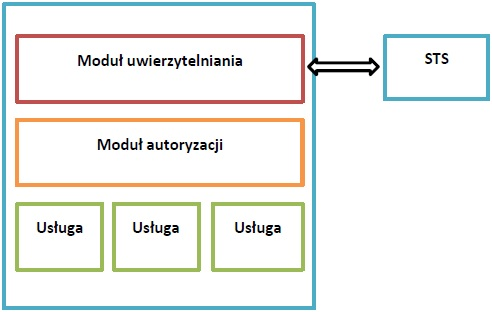
\includegraphics{img/interceptorGateway.jpg}
			\caption{Zastosowanie wzorca ,,Message Interceptor Gateway'' w procesie uwierzytelniania klienta serwisu webowego}
			\label{Zastosowanie wzorca ,,Message Interceptor Gateway'' w procesie uwierzytelniania klienta serwisu webowego}
		\end{figure}

		Zastosowanie wzorca wprowadza do systemu pojedynczy punkt weryfikacji uprawnień klienta do żądanych zasobów. Gwarantuje w ten sposób, że wszystkie zasoby w ramach jednej domeny będą odpowiednio chronione i każde żądanie użytkownika usługi przejdzie tą samą ścieżkę weryfikacji uprawnień przed przyznaniem prawa dostępu do funkcjonalności usługi. Obsługa żądań klientów rozpoczyna się od uwierzytelnienia klienta. Uwierzytelnianie odbywa się na podstawie asercji SAML przesyłanej w nagłówku wiadomości. Otrzymana asercja jest weryfikowana przy użyciu usługi ,,Security Token Service''. Dzięki asercji uznanej w procesie weryfikacji za poprawną możliwe jest dostęp do informacji o użytkowniku, np. jego nazwy oraz ról do jakich jest przypisany. Żądanie uwierzytelnionego użytkownika poddawane jest kolejnej weryfikacji w module autoryzacji. Moduł sprawdza, czy dany klient jest uprawniony do korzystania z usługi, do której chce uzyskać dostęp. W zaproponowanych rozwiązaniach wykorzystywany jest model autoryzacji RBAC(Role Based Access Control). Prawa dostępu weryfikowane są na podstawie przynależności użytkownika do określonej roli. Gdy moduł autoryzacji potwierdza uprawnienia klienta do usługi, udostępniane są mu zasoby serwisu.

	\subsection{Uwierzytelnianie klientów usług webowych przy użyciu asercji SAML w architekturze SOA}


		Zastosowanie koncepcji systemów zarządzania tożsamościami w architekturze zorientowanej na usługi przedstawione zostało na przykładzie prostego systemu obsługi zamówień sklepu internetowego. Opracowane zostały różne usługi realizujące poszczególne etapy dokonywania zamówienia. Serwisy zaimplementowane zostały przy użyciu różnych standardów dostarczania usług webowych(REST i SOAP). Wykorzystują schemat przebiegu procesu uwierzytelniania opisany w rozdziale ,,Komponenty systemu uwierzytelniania klientów usług webowych w oparciu o standard SAML'' niniejszej pracy. Proces uwierzytelniania oparty jest na mechanizmach opisanych standardem WS-Trust - wykorzystuje usługę ,,Security Token Service''. Proces zamówienia realizowany jest przez usługi odpowiedzialne za sprawdzanie stanu magazynu, zlecenie dostawy towaru, zlecenie wydania towaru  oraz rejestrację transakcji w serwisie księgowym. Usługi zlokalizowane są w różnych domenach. Uwierzytelnianie klientów usług opiera się na otrzymywanych asercjach SAML i wykorzystuje mechanizm weryfikacji tokenów bezpieczeństwa dostarczany przez usługę STS. 

	\subsection{Komponenty przykładowego systemu obsługi zamówień}	
		
		Stworzony system obsługi zleceń w sklepie internetowym stanowi „proof of concept” niniejszej pracy. Ponieważ dostarczane przez niego funkcje nie są szczególnie istotne z punktu widzenia analizy mechanizmów bezpieczeństwa, zostaną one opisane bez szczegółowej analizy. StoresStateService jest usługą udostępniającą informacje na temat stanu magazynowego sklepu. Przyjmuje ona nazwę oraz ilość egzemplarzy zamówionego produktu, a odpowiedź usługi zawiera lokację magazynu który posiada wymagany towar. WarehouseService rejestruje zamówienie w magazynie, zwracając potwierdzenie rejestracji. FinancialDepartmentService obsługuje system fakturowania, który zwraca identyfikator faktury. Ostatnim komponentem funkcjonalnym jest DeliveryService, który ma stanowić usługę dostarczaną przez zewnętrznego partnera biznesowego sklepu. Przyjmuje ona informacje o planowanej przesyłce, zwracając systemowi identyfikator przesyłki. 
		
		\begin{figure}[h]
			\centering
			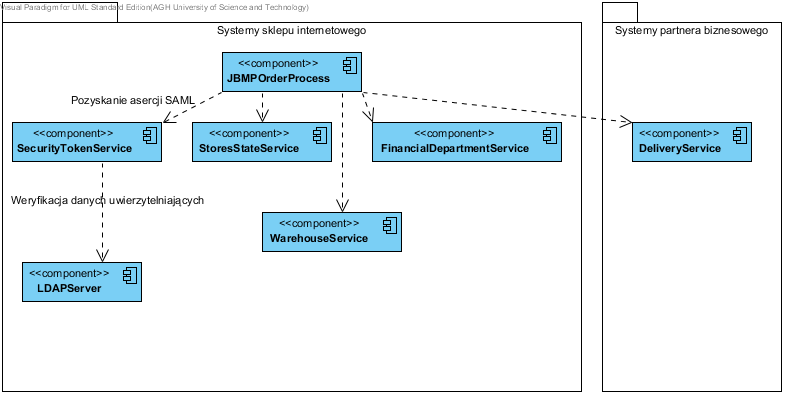
\includegraphics[width=\textwidth]{img/KomponentySystemu.png}
			\caption{Diagram komponentów przykładowego systemu obsługi zamówień}
			\label{Komponenty}
		\end{figure}	
		
%---------------------------------------------------------------------------

\section{Środowisko wdrożenia}
\label{sec:srodowiskoWdrozenia}

Jednym z wymagań pracy było uruchomienie stworzonego przykładowego systemu w środowisku chmury obliczeniowej. Ponieważ system ten był tworzony przy użyciu standardowych i dobrze wspieranych narzędzi(język programowania i biblioteki), naturalnym wyborem było wykorzystanie modelu Platform as a Service. Model pozwala na łatwiejsze wdrożenie aplikacji w porównaniu z IaaS, zachowując poziom elastyczności wymagany do zrealizowania postawionych wymagań projektowych, w przeciwieństwie do SaaS.

Użycie chmury obliczeniowej pozwala na łatwe przenoszenie poszczególnych komponentów pomiędzy serwerami i dynamiczne tworzenie domen bezpieczeństwa, pozwalając tym samym na przetestowanie zachowania systemu w środowisku wielodomenowym. Większość komponentów systemu może być uruchomiona wewnątrz jednego serwera aplikacji, w tej samej domenie bezpieczeństwa. Z punktu widzenia modelowania środowiska wielodomenowego, istotne jest jedynie to aby przynajmniej jeden komponent znalazł się w osobnej domenie.
Wykorzystane środowisko powinno udostępniać możliwość zewnętrznej komunikacji z wykorzystaniem protokołu HTTP, w celu udostępnienia usług sieciowych opartych o wzorzec REST i protokół SOAP. Chmura musi także umożliwiać komunikację pomiędzy usługą Security Token Service i serwerem LDAP. Z powodu ograniczeń technicznych serwer LDAP został uruchomiony na innym węźle niż tym na którym jest pracuje serwer aplikacji z systemem obsługi sklepu internetowego.
Końcową strukturę wdrożenia systemu obrazuje poniższy diagram.

		\begin{figure}[h]
			\centering
			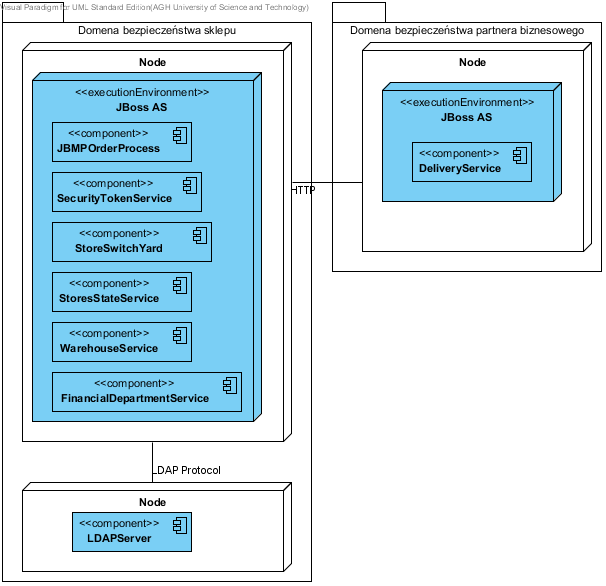
\includegraphics{img/DeploymentDiagram1.png}
			\caption{Diagram wdrożenia przykładowego systemu obsługi zamówień w środowisku chmury obliczeniowej}
			\label{DeploymentDiagram}
		\end{figure}

%---------------------------------------------------------------------------

\section{Zastosowane mechanizmy integracji}
\label{sec:integracja}

		\begin{figure}[h]
			\centering
			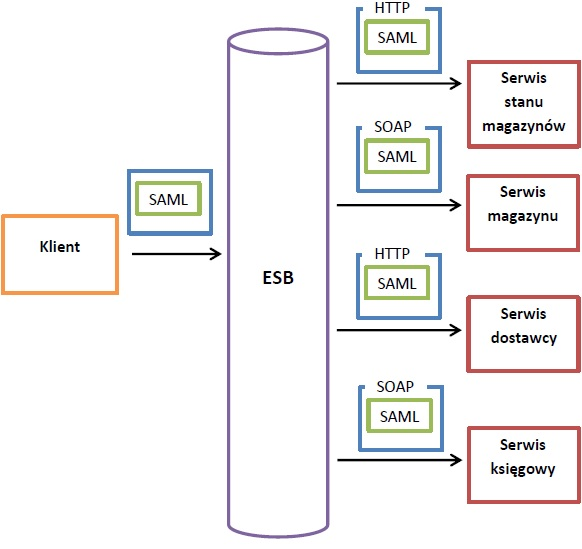
\includegraphics{img/esbAndSAML.jpg}
			\caption{Udział magistrali ESB w procesie wywołań usług z mechanizmami uwierzytelniania opartymi o SAML}
			\label{ESB i SAML}
		\end{figure}

		Do architektury proponowanego systemu wprowadzono dodatkową warstwę - magistralę usług(Enterprise Serial Bus). Magistrala usług pośredniczy w wywołaniach usług udostępnianych przez serwisy - otrzymuje wiadomości wraz z załączonymi tokenami bezpieczeństwa kierowane do przyłączonych serwisów. 
		
		Ponieważ klient serwisu odnosi się wyłącznie magistrali usług w celu skorzystania z usługi, nie musi on nic wiedzieć o rzeczywistym dostawcy usługi. Zapewnia to przezroczystość lokalizacji(ang. location transparency), która jest szczególnie istotna w środowisku chmury obliczeniowej, w którym rzeczywista lokacja usługi może dynamicznie się zmieniać. Podejście to ułatwia także zapewnienie skalowalności poprzez umożliwienie zwielokrotnienia instancji dostawców usług.
		Jednym z głównych cech większości rozwiązań typu ESB jest pośredniczenie w transformacji wiadomości i konwersji protokołów pomiędzy nadawcą a odbiorcą wiadomości. Magistrala dostosowuje otrzymywane wiadomości do formatu wykorzystywanego przez daną usługę. W przypadku stworzonego przykładowego systemu obsługi zamówień, magistrala udostępnia zasoby REST stanowiące interfejs kliencki do usług realizowanych przez serwisy uruchomione w systemie.
		
		Zadania magistrali usług w kontekście obsługi tokenów bezpieczeństwa są ograniczone. Moduł ESB nie dokonuje analizy ani przetwarzania otrzymywanych asercji SAML. Jedynym zadaniem magistrali w procesie obsługi tokenów bezpieczeństwa jest dołączenie tokenu do nagłówka odpowiedniego typu dla danego formatu wiadomości akceptowanych przez usługę.
		Strukturę komponentów po wprowadzeniu magistrali usług przedstawia poniższy diagram.

		\begin{figure}[h]
			\centering
			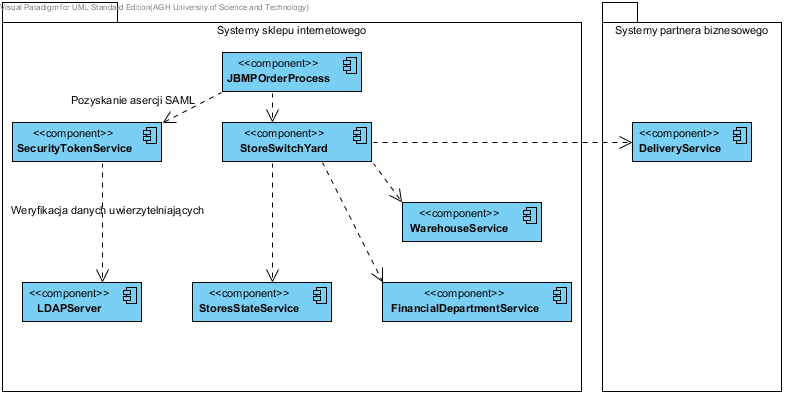
\includegraphics[width=\textwidth]{img/KomponentySystemuESB.png}
			\caption{Diagram komponentów przykładowego systemu obsługi zamówień z wykorzystaniem ESB}
			\label{KomponentyESB}
		\end{figure}
		
%---------------------------------------------------------------------------
